%!TEX TS-program = pdflatex

\documentclass[a4paper,8pt]{article} % добавить leqno в [] для нумерации слева

\usepackage[left=2cm,right=2cm,
top=2cm,bottom=2cm,bindingoffset=0cm]{geometry}

\usepackage[english, russian]{babel} % выбор языка для документа
\usepackage[utf8]{inputenc} % задание utf8 кодировки исходного tex файла
%\usepackage[T1,T2A]{fontenc}        % кодировка

%\usepackage{fontspec}         % пакет для подгрузки шрифтов
%\setmainfont{Times New Roman}       % задаёт основной шрифт документа

\usepackage{multirow}

\usepackage{amsmath,amsfonts,amssymb,amsthm,mathtools} % AMS
\usepackage{icomma} 
\mathtoolsset{showonlyrefs=true} % Показывать номера только у тех формул, на которые есть \eqref{} в тексте.
%\usepackage{euscript}	 % Шрифт Евклид
%\usepackage{mathrsfs} % Красивый матшрифт
\usepackage{enumitem}
\usepackage{siunitx}
\usepackage{tikz} % To generate the plot from csv
\usepackage{pgfplots}

\usepackage{hyperref}

%%% Заголовок

\newcommand{\latinword}[1]{\textsf{\itshape #1}}%


\usepackage{indentfirst}
\usepackage{fancyvrb}

\usepackage{graphicx} 
\usepackage{float}

\usepackage{mathtools}

%\usepackage[noae]{Sweave}

\usepackage[backend=biber, maxbibnames=9,maxcitenames=2,uniquelist=false]{biblatex}


\addbibresource{bibl.bib} % сюда нужно вписать свой bib-файлик.


\pgfplotsset{compat=1.17} 


\begin{document}
	

\subsection*{Микроэкономика}

\textbf{Тема 1. Поведение потребителей:
спрос.}

1)

Наклон бюджетной линии на плоскости
$\left(x_{1}, x_{2}\right)$ равен $-\frac{p_{1}}{p_{2}} .$

Определение.
Пусть при ценах $p=\left(p_{1}, p_{2}\right)$ потребитель приобрел набор $x=\left(x_{1}, x_{2}\right) .$ Тогда набор $x=\left(x_{1}, x_{2}\right)$ 
выявленно предпочитается,  если 
$p_{1} y_{1}+p_{2} y_{2} \leq p_{1} x_{1}+p_{2} x_{2} .$

WARP: Если набор $x$ выявленно предпочитается набору $y$ и $x \neq y,$ то набор $y$ не может выявленно предпочитаться набору $x$.

Формально: пусть при ценах $p=\left(p_{1}, p_{2}\right)$ потребитель выбрал набор $x=\left(x_{1}, x_{2}\right),$ а при ценах $q=\left(q_{1}, q_{2}\right)$ потребитель выбрал набор $y=\left(y_{1}, y_{2}\right), x \neq y .$ Тогда поведение потребителя
согласуется с WARP, если из $p_{1} x_{1}+p_{2} x_{2} \geq p_{1} y_{1}+p_{2} y_{2},$ следует $q_{1} y_{1}+q_{2} y_{2}<q_{1} x_{1}+q_{2} x_{2} . $

Если, приобретая набор $x=\left(x_{1}, x_{2}\right)$ при ценах $p=\left(p_{1}, p_{2}\right),$ потребитель не мог купить набор
$y=\left(y_{1}, y_{2}\right),$ а при выборе набора $y=\left(y_{1}, y_{2}\right)$ при ценах $q=\left(q_{1}, q_{2}\right),$ набор $x=\left(x_{1}, x_{2}\right)$ был не
доступен, то будет говорить, что такое поведение не противоречит WARP, и наборы $x=\left(x_{1}, x_{2}\right)$
и $y=\left(y_{1}, y_{2}\right)$ выявленно несравнимы.

2) Свойства предпочтений: полнота, транзитивность, непрерывность. 

Предельная норма замещения равна наклону кривой безразличия в пространстве благ $\left(x_{1}, x_{2}\right),$ взятому с обратным знаком: $M R S_{12}(x)=-\frac{d x_{2}}{d x_{1}}$ ($M R S_{12}(x)=\frac{\partial u(x) / \partial x_{1}}{\partial u(x) / \partial x_{2}}$.)

Функция полезности Кобба-Дугласа: $u\left(x_{1}, x_{2}\right)=x_{1}^{\alpha} x_{2}^{\beta}, \alpha, \beta>0$ (или любое положительной преобразование этой функции).  $M R S_{12}\left(x_{1}, x_{2}\right)=\frac{\alpha x_{2}}{\beta x_{1}}$

$x_{1}\left(p_{1}, p_{2}, m\right)=\frac{\alpha m}{(\alpha+\beta) p_{1}}, x_{2}\left(p_{1}, p_{2}, m\right)=\frac{\beta m}{(\alpha+\beta) p_{2}}$

Если предпочтения потребителя строго монотонны, функция полезности дифференцируема и $\tilde{x}=\left(\tilde{x}_{1}, \tilde{x}_{2}\right)$ - внутреннее решение задачи потребителя, то $M R S_{12}(\tilde{x})=\frac{p_{1}}{p_{2}} .$


Кривая Энгеля ($Y\mid Q$).

По Слуцкому: 
$\frac{\Delta x}{\Delta p}=\left.\frac{\Delta x}{\Delta p}\right|_{M=\text { const }}+\frac{\Delta x}{\Delta M} \frac{\Delta M}{\Delta p}=\left.\frac{\Delta x}{\Delta p}\right|_{M=c o n s t}-x \frac{\Delta x}{\Delta M}$
поскольку изменение реального дохода $\Delta M=-x \Delta p$ (трактовка Слуцкого).

$E_{P}^{D}=\frac{\Delta Q / Q}{\Delta P / P}$,
$E_{I}^{D}=\frac{\Delta Q / Q}{\Delta I / I}$, $E_{X Y}^{D}=\frac{\Delta Q_{X} / Q_{X}}{\Delta P_{Y} / P_{Y}}$


\textbf{Тема 2. Теория производства. Поведение фирмы, максимизирующей
прибыль.}

Предельная норма технологического замещения характеризует
тангенс угла наклона касательной к изокванте (с обратным знаком)
$\operatorname{MRTS}_{12}\left(x_{1}, x_{2}\right)=\frac{M P_{1}\left(x_{1}, x_{2}\right)}{M P_{2}\left(x_{1}, x_{2}\right)}$

Если производственная функция дифференцируема, то в краткосрочном периоде $p M P_{1}\left(\tilde{x}_{1}, \bar{x}_{2}\right)=w_{1} .$ 

Если производственная функция дифференцируема, то в долгосрочном периоде
$\operatorname{MRTS}_{12}\left(\tilde{x}_{1}, \tilde{x}_{2}\right)=\frac{w_{1}}{w_{2}} .$ Если производственная функция вогнута, то условие $\operatorname{MRTS}_{12}\left(\tilde{x}_{1}, \tilde{x}_{2}\right)=\frac{w_{1}}{w_{2}}$


\textbf{Тема 3. Конкурентные и неконкурентные рынки и особенности их
функционирования.}

Индекс Лернера: $I_{L}=\frac{P_{m}-M C}{P_{m}}=\frac{1}{E}$


\textbf{Тема 4. Рынки факторов производства и особенности их функционирования.}

Поведение индивида на рынке труда. 
Условие оптимального выбора между потреблением и отдыхом: равенство предельной нормы замещения потребления трудом и предельного продукта труда. 

Поведение фирмы на рынке труда. Предельная доходность труда (предельная отдача от труда в денежном выражении). Предельные затраты на найм
работников. Условие максимизации прибыли фирмы на рынке труда.

Максимизация прибыли фирмой на рынке
капитала. Равенство предельной доходности капитала и издержек
привлечения единицы капитала. 

Связь между инвестициями и доходностью
финансовых активов. Ставка процента как альтернативные затраты
инвестиций в реальный сектор. Рыночная стоимость фирмы. Коэффициент
qДж.Тобина. Теория акселератора инвестиций.

\newpage

\subsection*{Макроэкономика}


\textbf{Тема 1. Введение в макроэкономику. Основные
макроэкономические показатели производства, доходов и
цен.}

Изъятия и инъекции. Основное макроэкономическое тождество: Y = C + I + G + NX (равенство доходов и расходов).

Уравнение Фишера: $r=\frac{i-\pi^{e}}{1+\pi^{e}}$,  $i=r+\pi^{e}$

Уровень безработицы: $u=\frac{U}{L} \times 100 \% \quad$ или $\quad u=\frac{U}{E+U} \times 100 \%$

Номинального и реального валютного курса: $E_{R}=E_{N} \times \frac{P_{d}}{P_{f}}$

Закон единой цены
$
P_{i}^{f}=P_{i}^{d} E^{f / d}
$

Абсолютный РРР
$
E^{f / d}=\frac{P^{f}}{P^{d}}
$

Относительный РРР в темповой записи
$
e^{f / d}=g_{E}=\pi^{f}-\pi^{d}
$


\textbf{Тема 2. Равновесие на товарном рынке. Фискальная политика и
ее воздействие на экономику.}

Модель ``Кейнсианского креста'' ($AE \mid Y$). 

Фискальная политика: цели, инструменты: G, T, Tr. 

Автоматические стабилизаторы - это инструменты доходов и расходов государственного бюджета, которые автоматически меняются в зависимости от состояния экономики таким образом, что ВВП стабилизируется (трансферты; личные подоходные налоги;
налоги на прибыль корпораций; НДС и т.п.) 

Налоговый мультипликатор:  $\Delta Y=\frac{1}{1-m p c}(-m p c \cdot \Delta \bar{T}) \Delta Y=-\frac{m p c}{1-m p c} \Delta \bar{T}$  (трансфертов: $\Delta Y=\frac{m p c}{1-m p c}  \Delta \underline{T r} .$)

Мультипликатор государственных закупок: $\Delta Y_{G}=\frac{1}{1-m p c} \Delta \underline{G}$

Бюджетный мультипликатор:  $\Delta Y=\frac{1}{1-m p c} \Delta \underline{G}+\frac{-m p c}{1-m p c} \Delta \underline{T} = 1$, поскольку бюджет сбалансированный

Модель IS ($r \mid Y$)


\textbf{Тема 3. Равновесие на денежном рынке. Монетарная
политика.}

Количественная теория денег: $M V=P Q$

Теория предпочтения ликвидности: $M^{D}=M_{S}^{D}+M_{T}^{D}+M_{P}^{D}=f(i, Y)$



$\mathrm{M} (денежная масса)   =  C (наличность) + D (депозит)$

$\mathrm{H} (денежная база) = С + R (обяз. резерервы)$

$\mathrm{rr}=\mathrm{R} / \mathrm{D} \quad \mathrm{R}=\mathrm{rr}^{*} \mathrm{D}$

$\mathrm{cr}=\mathrm{C} / \mathrm{D} \quad \mathrm{C}=\mathrm{cr}^{*} \mathrm{D}$

$\mathrm{M}=\mathrm{C}+\mathrm{D}=\mathrm{cr}^{*} \mathrm{D}+\mathrm{D}=(\mathrm{cr}+1) \mathrm{D}$

$H=C+R=c r^{\star} D+r r^{*} D=(c r+r r) D$

$m=\frac{M}{H}=\frac{c r+1}{c r+r r}$ 


Денежный рынок (r|(M/P))

Инструменты монетарной политики: (покупка/продажа ценных бумаг;  нормы обязательных резервов; учетная  ставка) 



Кривая LM ($r\mid Y)$.




\textbf{Тема 4. Анализ экономики с жесткими и гибкими ценами. Модель
AD-AS.}


\begin{figure}[h]
	\centering
	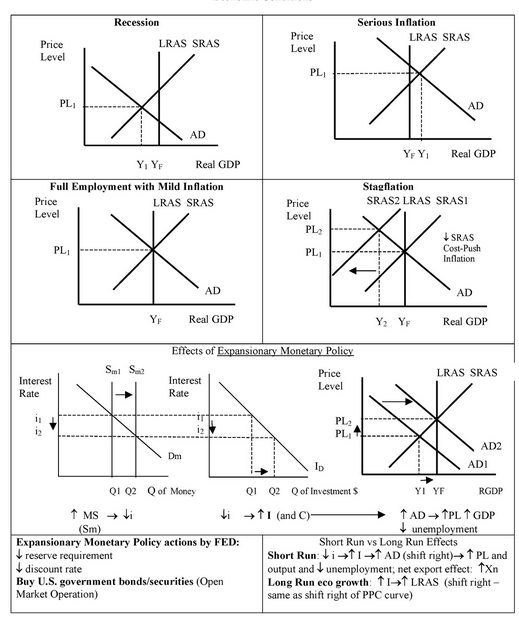
\includegraphics[width=0.7\linewidth]{screenshot003}
%	\caption{}
	\label{fig:screenshot003}
\end{figure}



\textbf{Тема 5. Экономические колебания. Экономический
рост.}

Закон Оукена \textsf{}

$\frac{Y-Y *}{Y *}=-B u_{c}$

где Y — фактический ВВП, Y* — потенциальный ВВП, $u_c$ — уровень циклической безработицы, B — эмпирический коэффициент чувствительности (обычно принимается 2). 

Следствие из закона Оукена:
$$
\frac{Y_{1}-Y_{0}}{Y_{0}}=-\frac{B\left(u_{1}-u_{0}\right)}{1-B u_{0}}
$$

$Y_{1}, u_{1}-$ ВНП и уровень безработицы в текущем периоде
$Y_{0}, u_{0}-$ ВНП и уровень безработицы в базовом периоде

Формально современная кривая Филлипса записывается следующим образом: $\pi=\pi_{e}-b\left(u-u_{e}\right)+v,$ где
$-\pi-$ уровень инфляции,
- $\pi_{e}$ - ожидаемый уровень инфляции,
$-\left(u-u_{e}\right)-$ отклонение безработицы от естественного уровня - циклическая безработица,
- $b>0$ - коэффициент, чувствительности инфляции к отклонению безработицы,
- $v$ - шок предложения.


$\dot{K}=s Y_{t}-\delta K_{t}$, $k=\frac{K}{L E}$, $\frac{\dot{L}}{L_{t}}=n$, $\frac{\dot{E}}{E_{t}}=g$


$\dot{k}=\frac{\dot{K}}{L_{t} E_{t}}-\frac{K_{t}\left(\dot{L} E_{t}+L_{t} \dot{E}\right)}{\left(L_{t} E_{t}\right)^{2}}=\frac{s Y_{t}-\delta K_{t}}{L_{t} E_{t}}-\frac{K}{L E}\left(\frac{\dot{L}}{L_{t}}+\frac{\dot{E}}{E_{t}}\right)=s f\left(k_{t}\right)-(n+g+\delta) k_{t}$

В стационарном состоянии темп прироста показателей на единицу эффективного труда равен нулю
$$
\frac{\dot{y}}{y}=g_{y}=\frac{\dot{c}}{c}=g_{c}=\frac{\dot{k}}{k}=g_{k}=0 .
$$
Показатели на единицу труда растут с темпом технологического прогресса $g$
$$
\frac{\left(\frac{\dot{Y}}{L}\right)}{\frac{Y}{L}}=g_{Y / L}=\frac{\left(\frac{\dot{C}}{L}\right)}{\frac{C}{L}}=g_{C / L}=\frac{\left(\frac{\dot{K}}{L}\right)}{\frac{K}{L}}=g_{K / L}=g
$$
Валовые показатели растут с темпом равным сумме темпов прироста технологического прогресса $g$ и населения $n$
$$
\frac{\dot{Y}}{Y}=g_{Y}=\frac{\dot{C}}{C}=g_{C}=\frac{\dot{K}}{K}=g_{K}=g+n
$$

``Золотое правило''

$\max _{s} c[k(s)]$ при условии:
$
\dot{k}=0
$


$c[k(s)]=(1-s) y=f[k(s)]-(n+g+\delta) k(s)$

$\frac{\partial c}{\partial s}=0$
Значит, в точке максимума должно выполняться равенство
 $\frac{\partial f\left(k^{* *}\right)}{\partial k}=n+g+\delta$
где $k^{* *}-$ устойчивый уровень капиталовооружённости на единицу эффективного труда, соответствующий максимальному потреблению.

Таким образом, норма сбережений $s^{*}$, максимизирующая потребление $c$, находится из решения системы уравнений:
$$
\left\{\begin{array}{l}
s^{*} f\left(k^{* *}\right)=(n+g+\delta) k^{* *} \\
\frac{\partial f\left(k^{* *}\right)}{\partial k}=n+g+\delta
\end{array}\right.
$$

В результате решения этой системы оптимальная норма сбережения, соответствующие «Золотому правилу», равна эластичности выпуска по капиталу:  $s^{*}=\frac{k^{* *}}{f\left(k^{* *}\right)} \times \frac{\partial f\left(k^{* *}\right)}{\partial k} .$

\newpage

\hypertarget{ux44dux43aux43eux43dux43eux43cux435ux442ux440ux438ux43aux430}{%
\subsection*{Эконометрика}}

\textbf{Тема 1. Теория вероятностей:}


The joint CDF of $X$ and $Y$ is
$
F(x, y)=P(X \leq x, Y \leq y)
$ 
or $
p_{X, Y}(x, y)=P(X=x, Y=y)
$

In the continuous case, they have a joint PDF
$
f_{X, Y}(x, y)=\frac{\partial^{2}}{\partial x \partial y} F_{X, Y}(x, y)
$



\begin{figure}[H]
\centering
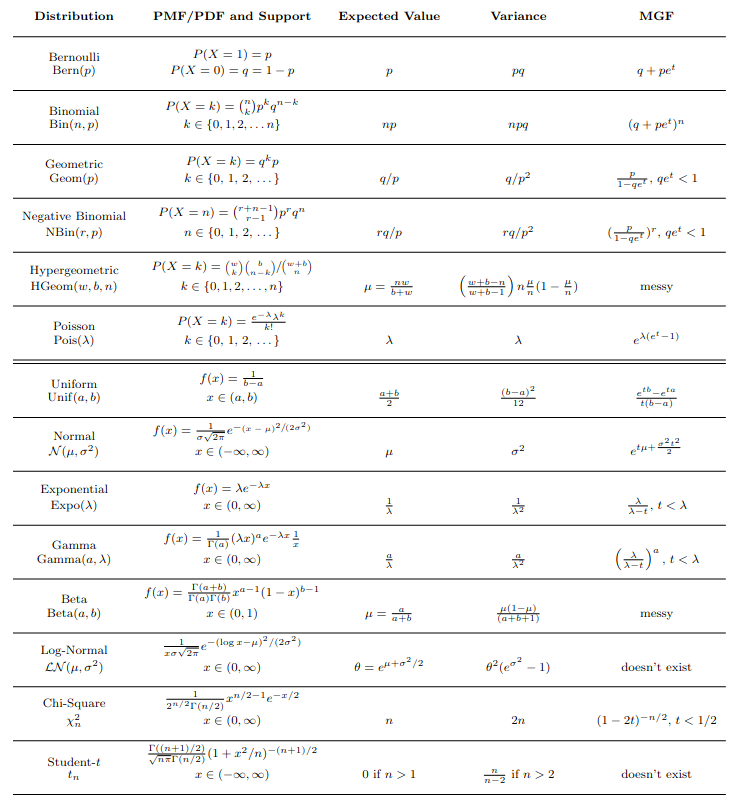
\includegraphics[width=0.9\linewidth]{screenshot001}
%	\caption{}
\label{fig:screenshot001}
\end{figure}

Conditional Distributions
Conditioning and Bayes' rule for discrete r.v.s
$$
P(Y=y \mid X=x)=\frac{P(X=x, Y=y)}{P(X=x)}=\frac{P(X=x \mid Y=y) P(Y=y)}{P(X=x)}
$$
Conditioning and Bayes' rule for continuous r.v.s
$$
f_{Y \mid X}(y \mid x)=\frac{f_{X, Y}(x, y)}{f_{X}(x)}=\frac{f_{X \mid Y}(x \mid y) f_{Y}(y)}{f_{X}(x)}
$$
Hybrid Bayes' rule
$$
f_{X}(x \mid A)=\frac{P(A \mid X=x) f_{X}(x)}{P(A)}
$$

\newpage

\textbf{Тема 2. Математическая
статистика:}

\begin{figure}[H]
\centering
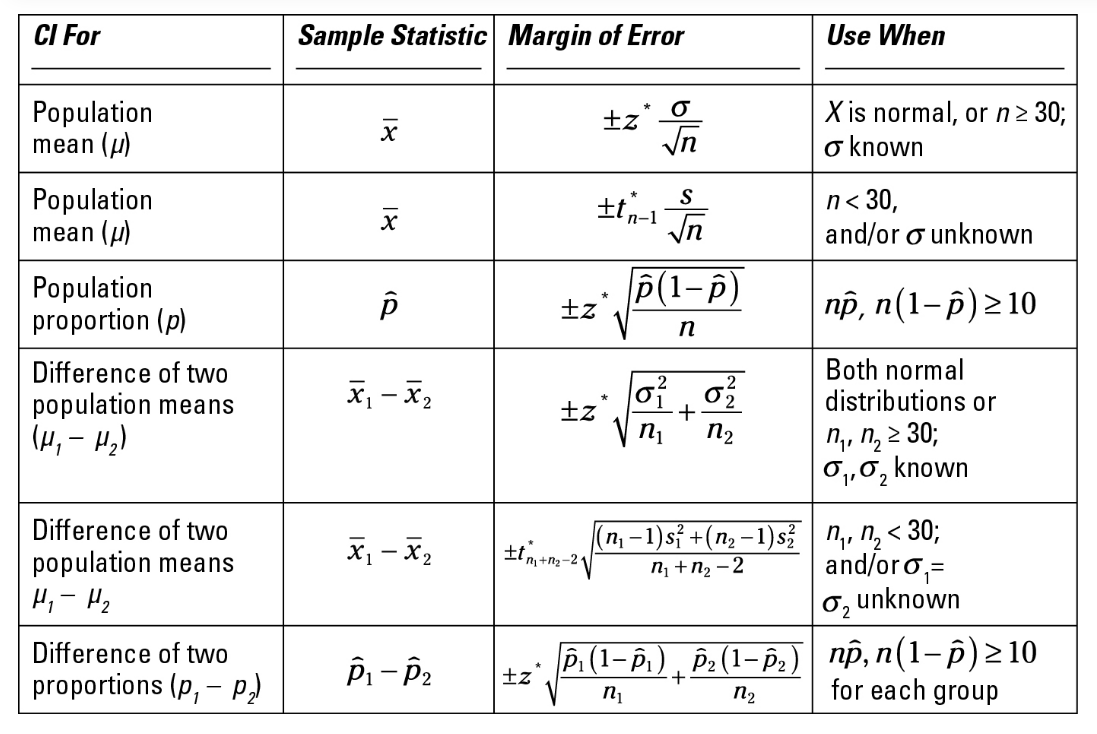
\includegraphics[width=0.7\linewidth]{screenshot002}
%	\caption{}
\label{fig:screenshot002}
\end{figure}

% Please add the following required packages to your document preamble:
% \usepackage{multirow}
\begin{table}[H]
\begin{tabular}{|c|c|c|c|}
\hline
\multicolumn{2}{|c|}{\multirow{2}{*}{}} & \multicolumn{2}{c|}{Null hypothesis $\left(H_{0}\right)$ is} \\ \cline{3-4} 
\multicolumn{2}{|c|}{} & True & False \\ \hline
\multirow{2}{*}{\begin{tabular}[c]{@{}c@{}}Decision\\ about null\\ hypothesis $\left(H_{0}\right)$\end{tabular}} & \begin{tabular}[c]{@{}c@{}}Don't\\ reject\end{tabular} & \begin{tabular}[c]{@{}c@{}}True Negative\\ Confidence:\\ $P\left(S^{obs} \not\subset D^{crit} \mid H_{0}\right)=1-\alpha$\end{tabular} & \begin{tabular}[c]{@{}c@{}}False Negative\\ Type II error:\\ $P\left(S^{obs} \not\subset D^{crit} \mid H_{1}\right)=\beta$\end{tabular} \\ \cline{2-4} 
& Reject & \begin{tabular}[c]{@{}c@{}}False Positive\\ Type I error: \\ $P\left(S^{obs} \subset D^{crit} \mid H_{0}\right)=\alpha$\end{tabular} & \begin{tabular}[c]{@{}c@{}}True Positive\\ Power:\\ $P\left(S^{obs} \subset D^{crit} \mid H_{1}\right)=1-\beta$\end{tabular} \\ \hline
\end{tabular}
\end{table}


\newpage

\textbf{Тема 3. Линейная регрессионная модель для случая одной объясняющей переменной} 

$$
\begin{aligned}
\hat{\beta}_{0} &=\bar{y}-\hat{\beta}_{1} \bar{x} \\
\hat{\beta}_{1} &=\frac{\widehat{\operatorname{Cov}}(y, x)}{\widehat{\operatorname{Var}}(x)}
\end{aligned}
$$

$\sum_{i=1}^{N} \hat{u}_{i}=0$ (mean \& sum of residuals is zero) 

$\sum_{i=1}^{N} x_{i} \hat{u}_{i}=0$ (zero covariance bet. $x$ and resids. $)$ 

The OLS line (SRF) always passes through $(\bar{x}, \bar{y})$ 

Variance and Standard Error of $\hat{\beta}_{i}$
$$
\operatorname{Var}\left(\hat{\beta}_{j}\right)=\frac{\sigma^{2}}{S S T_{j}\left(1-R_{j}^{2}\right)}, j=1,2, \ldots, k
$$
where
$$
S S T_{j}=(N-1) \operatorname{Var}\left(x_{j}\right)=\sum_{i=1}^{N}\left(x_{i j}-\bar{x}_{j}\right)
$$
$R_{j}^{2}=R^{2}$ from a regression of $x_{j}$ on all other $x$ 's Standard deviation: $\quad \sqrt{\operatorname{Var}}$
Standard error:
$$
\sqrt{\widehat{V a r}}
$$
$$
\operatorname{se}\left(\hat{\beta}_{j}\right)=\sqrt{\frac{\hat{\sigma}^{2}}{S S T_{j}\left(1-R_{j}^{2}\right)}}, j=1, \ldots, k
$$



\textbf{Тема 4. Дисперсионный
анализ
}


$\quad TS S=\sum_{i=1}^{N}\left(y_{i}-\bar{y}\right)^{2}$, $ES S =\sum_{i=1}^{N}\left(\hat{y}_{i}-\bar{y}\right)^{2}$, 
$RS S =\sum_{i=1}^{N} \hat{u}_{i}^{2}$,  $ES S +RS S =TS S $

$R^{2}=\frac{ESS}{TS S} $, 
$0 \leq R^{2} \leq 1$, 
$R^2_{UC} = 1 - \frac{RSS}{\sum y_i^2}  = \frac{\sum\hat{y}_i^2}{\sum y_i^2} $, $R^2_{adj} = 1 - \frac{n-1}{n-k-1} \frac{RSS}{TSS} = 1 - \frac{s^2_{\hat{u}}}{s^2_{y}}$ 



$\hat{\sigma}^{2} =\frac{S S R}{N-K-1} =\frac{1}{N-K-1} \sum_{i=1}^{N} \hat{u}_{i}^{2}$






\textbf{Тема 5. Матричная форма. Теорема Гаусса-Маркова}

$\hat{\beta}=\left(X^{\prime} X\right)^{-1} X^{\prime} y$



$\hat{\sigma}^{2}=\frac{e^{\prime} e}{n-k}$

$\hat{\beta} \sim N\left[\beta, \sigma^{2}\left(X^{\prime} X\right)^{-1}\right]$

\textbf{Тема 6. Проверка гипотезы об адекватности регрессии.
Проверка гипотезы о линейных ограничениях на коэффициенты
регрессии}


\textit{F-test for regression fit: }

$H_0: \beta_1 = \dots = \beta_{k-1} = 0  $

$H_a: \text{at least one } \beta_j \neq 0, j=1,\dots,k-1  $

$F=\frac{E S S /(k-1)}{R S S /(n-k)} =\frac{R^2 /(k-1)}{(1-R^2) /(n-k)} \sim F(k-1,n-k)$

\textit{RESET test:}


$H_0: \gamma_1 = \dots = \gamma_q = 0  $

$H_a: \text{ at least one } \gamma_j \neq 0, j=1,\dots,q  $

$F=\frac{\left( RSS_{R}-RSS_{UR}\right) / q}{RSS_{UR} /(n-k-q)}=\frac{\left( R^2_{UR}-R^2_{R}\right) / q}{(1- R^2_{UR}) /(n-k-q)} \sim F(q,n-k-q) $




\textbf{Тема 7. Функциональные преобразования переменных в линейной регрессионной модели.}

\begin{equation}
\begin{array}{lccc}
\hline \text { Model } & \text { DV } & \text { RHS } & \text { Interpretation of } \beta_{1} \\
\hline \text { Level-level } & y & x & \Delta y=\beta_{1} \Delta x \\
\text { Level-log } & y & \log (x) & \Delta y=\left(\beta_{1} / 100\right)[1 \% \Delta x] \\
\text { Log-level } & \log (y) & x & \% \Delta y=\left(100 \beta_{1}\right) \Delta x \\
\text { Log-log } & \log (y) & \log (x) & \% \Delta y=\beta_{1} \% \Delta x \\
\text { Quadratic } & y & x+x^{2} & \Delta y=\left(\beta_{1}+2 \beta_{2} x\right) \Delta x \\
\hline
\end{array}
\end{equation}





\textbf{Тема 8. Фиктивные переменные. Тест Чоу}

\textit{Chow test:}

$H_0: \beta_0^A  = \beta_0^B,   \dots , \beta_k^A  = \beta_k^B $

$H_a: \text{ at least one  of the restrictions is not hold }  $

$F=\frac{\left(R S S_{P}-R S S_{A}-R S S_{B}\right) / k}{\left(R S S_{A}+R S S_{B}\right) /(n-2 k)}  =  
\sim F(k,n-2k) $


\textbf{Тема 9. Мультиколлинеарность данных и способы борьбы с
ней}

$x_i \mid X_{-i}$,  $\mathrm{VIF}_{i}=\frac{1}{1-R_{i}^{2}}$,  If >10 hence MC

% Add a bibliography block to the postdoc


	
\end{document}
